% arara: pdflatex
% arara: bibtex
% arara: pdflatex
% arara: pdflatex
% 
% Annual Cognitive Science Conference
% Sample LaTeX Paper -- Proceedings Format
% 

% Original : Ashwin Ram (ashwin@cc.gatech.edu)       04/01/1994
% Modified : Johanna Moore (jmoore@cs.pitt.edu)      03/17/1995
% Modified : David Noelle (noelle@ucsd.edu)          03/15/1996
% Modified : Pat Langley (langley@cs.stanford.edu)   01/26/1997
% Latex2e corrections by Ramin Charles Nakisa        01/28/1997 
% Modified : Tina Eliassi-Rad (eliassi@cs.wisc.edu)  01/31/1998
% Modified : Trisha Yannuzzi (trisha@ircs.upenn.edu) 12/28/1999 (in process)
% Modified : Mary Ellen Foster (M.E.Foster@ed.ac.uk) 12/11/2000
% Modified : Ken Forbus                              01/23/2004
% Modified : Eli M. Silk (esilk@pitt.edu)            05/24/2005
% Modified : Niels Taatgen (taatgen@cmu.edu)         10/24/2006
% Modified : David Noelle (dnoelle@ucmerced.edu)     11/19/2014

%% Change "letterpaper" in the following line to "a4paper" if you must.

\documentclass[10pt,letterpaper]{article}
 
\usepackage{hyperref}
\usepackage{cogsci}
\usepackage{pslatex}
\usepackage{amsfonts}
\usepackage{graphicx}
\usepackage{apacite}
\usepackage{color}
\usepackage{todonotes}
\usepackage{dsfont}
\usepackage{textcomp}

\definecolor{Red}{RGB}{255,0,0}
\newcommand{\red}[1]{\textcolor{Red}{#1}}

\newcommand{\jd}[1]{\green{$^*$}\marginpar{\footnotesize{JD: \green{#1}}}}

\newcommand{\subsubsubsection}[1]{{\em #1}}
\newcommand{\eref}[1]{(\ref{#1})}
\newcommand{\tableref}[1]{Table \ref{#1}}
\newcommand{\figref}[1]{Figure \ref{#1}}
\newcommand{\appref}[1]{Appendix \ref{#1}}
\newcommand{\sectionref}[1]{Section \ref{#1}}

\title{Why do you ask? To be informative.}
 
\author{{\large \bf Robert X.~D.~Hawkins, Andreas Stuhlm\"uller, Judith Degen, Noah D.~Goodman}\\
  \{rxdh,astu,jdegen,ngoodman\}@stanford.edu\\
  Department of Psychology, 450 Serra Mall \\
  Stanford, CA 94305 USA}


\begin{document}

\maketitle


\begin{abstract}
aaaaaaaaaaaaaaaaaaaaaaaaaaaaaaaabstract
aaaaaaaaaaaaaaaaaaaaaaaaaaaaaaaabstract
aaaaaaaaaaaaaaaaaaaaaaaaaaaaaaaabstract
aaaaaaaaaaaaaaaaaaaaaaaaaaaaaaaabstract
aaaaaaaaaaaaaaaaaaaaaaaaaaaaaaaabstract
aaaaaaaaaaaaaaaaaaaaaaaaaaaaaaaabstract

\textbf{Keywords:} 
language understanding; pragmatics; Bayesian models; questions; answers
\end{abstract}

\section{Introduction}
\label{sec:intro}

% TODO:
% * refine example in intro paragraph -- something that better emphasizes 'question-as-signal'
% * design evocative cartoon for first page?
% * compress presentation of computational experiments; massage transition into behavioral experiment
% * incorporate discussion of paramter fitting 
% * include rigorous model comparison tests in results 
% *** (can we rule our the pragmatic questioner on the basis of model complexity?)
% * figure out whether related work section is worth the space, or if we want to factor into intro
% * think of other good discussion points

\begin{quote}
Q:``Are you gonna eat that?''
A:``Go ahead.''
\end{quote}
In this (real life) example, Q strategically chooses a question that differs from his true interest, avoiding an impolite question, yet manages to signal A about his interests; A in turn reasons beyond the overt question and provides an answer that addresses Q's interests.
This subtle interplay raises two questions for formal models of language:
What makes a question useful? What makes an answer appropriate? 
In this paper, we present three progressively more sophisticated computational models of question-answer behavior.
%, which formalize and probe the way answerers infer intentions and the way questioners signal them. 
We compare these models on the basis of two simulations of classic question-answer phenomena and one experiment in which participants must ask and answer questions in a communication game where we can experimentally manipulate the available questions and answers. 
We find that sophisticated pragmatic reasoning is needed to account for the data. This suggests that the purpose of questions in dialogue is to provide cues to the answerer about the questioner's interests; the appropriateness of an answer is the extent to which is informative about these interests.

%A:"can you pass he salt?"
%B:"yes (i am able)."

A number of studies in psycholinguistics have provided evidence that answerers are both sensitive to a questioner's goals and attempt to be informative with respect to those goals.
For instance, in the classic study of \citeA{Clark79_IndirectSpeechActs} researchers called liquor merchants and opened the conversation with one of two sentences to set context: ``I want to buy some bourbon'' (the \emph{uninformative} condition) or ``I've got \$5 to spend'' (the \emph{literal} condition). They then asked, ``Does a fifth of Jim Beam cost more than \$5?'' Merchants gave an exact price significantly more often in the uninformative context than the literal context, where a `yes' or `no' answer was more common. 
In the former case, the merchant inferred that the questioner's goal was just to buy whiskey, so the exact price was the maximally relevant response. In the latter case, the merchant inferred that the questioner's goal was to find out whether or not they could afford the whiskey, hence a simple `yes'  sufficed \cite{Clark79_IndirectSpeechActs}. 
Context and questioner goals have also been implicated in accounts of answers to identification questions like ``who is X?'' \cite{BoerLycan75_KnowingWho}, and to questions like ``where are you?'' that permit answers at many levels of abstraction \cite{Potts12_CardsDialogueCorpus}. While most of this work has focused on \emph{answerer} behavior, it suggests that the question itself is important in prompting a relevant answer.


%Suppose your friend asks you, ``Who is coming to the concert tonight?'' How do you respond? You certainly don't need to give the full list of attendees -- most of whom you do not know -- even though they would all technically be valid answers. Instead, you might only mention the set of \emph{mutual acquaintances} you know are planning to come, assuming that your friend doesn't care about the rest of the crowd. Now, imagine a different scenario. Suppose that you're waiting in line at the box office and want to find out whether your acquaintances had tickets as well. What question would you ask to the person in the ticket booth? If you asked, ``Who is coming to the concert tonight?''  you would likely get a quizzical look and an answer like ``A lot of people, why?'' because the person at the booth does not know your friends or your reason for asking the question. Instead, you might have to directly ask about your friends. Whether you're asking or answering questions, you must engage in some reasoning about the other person's intentions and knowledge. 
%
%Since both questioners and answerers appear to be acutely sensitive to one another's intentions and knowledge, what makes a question useful? What makes an answer to a question useful? In this paper, we present three progressively more sophisticated computational models of question-answer behavior, which formalize and probe this deep interaction between the way answerers infer intentions and the way questioners signal them. We compare these models on the basis of two simulations of classic question-answer phenomena and one experiment in which participants must ask and answer questions given a fixed set of goals. We find that a sophisticated pragmatic answerer is needed to account for the data, and close by proposing that the purpose of questions in dialogue is to provide cues to the answerer about the questioner's goals and intentions.

%A number of studies in psycholinguistics have provided evidence that answerers are both sensitive to a questioner's goals and attempt to be informative with respect to those goals. For example, when people are asked `Do you have the time?'' they typically round their answers to the nearest 5 or 10 minute interval, even when they're wearing a digital watch \cite{DerHenstCarlesSperber02_RelevanceTellingTime}. However, if the question is preceded by the statement ``My watch stopped,'' people make their response precise to the minute  \cite{GibbsBryant08_OptimalRelevance}. While an approximate time is sufficiently informative with respect to most goals, like making it to a meeting on time, this experiment demonstrated that answerers were able to infer that the goal of setting a watch required more precise information.

%Similar evidence comes from a classic study where researchers called liquor merchants and opened the conversation with one of two sentences: "I want to buy some bourbon'' (the `uninformative' condition) or ``I've got \$5 to spend'' (the `literal' condition) They then asked, ``Does a fifth of Jim Beam cost more than \$5?'' Merchants gave an exact price significantly more often in the `uninformative' context than the `literal' context, where a `yes' or `no' answer was more common. In the former case, the merchant inferred that the questioner's goal was just to buy whiskey, so the exact price was the maximally relevant response. In the latter case, the merchant inferred that the questioner's goal was literally to find out whether or not they could afford the whiskey, hence a simple `yes'  sufficed \cite{Clark79_IndirectSpeechActs}. Context and questioner goals have also been implicated in accounts of identification questions like ``who is X?'' \cite{BoerLycan75_KnowingWho}, and to questions like ``where are you?'' that permit answers at many levels of abstraction \cite{Potts12_CardsDialogueCorpus}. While most of this work has focused on \emph{answerer} behavior, it suggests that the question itself can signal the questioner's goals.


In this paper we extend the Rational Speech Act (RSA) framework \cite{frank2012, GoodmanStuhlmuller13_KnowledgeImplicature} for language understanding to address asking questions and giving answerers. The first challenge is that the speaker utility in this framework is usually identified with information provided---since questions don't provide direct information, we must say what utility they do have. We suggest, following \citeA{VanRooy03_QuestioningDecisionProblems}, that the value of a question is the extent to which it can be expected to provoke information relevant to the questioner \emph{later} in the dialogue. More specifically, the value of a question is the expected information about the interests of the questioner provided by the answer. This requires us to specify a model of the answerer---which can serve as both the model assumed by a questioner, and as a model of answer behavior itself.
We explore three, increasingly sophisticated, answerer models. The simplest answerer provides a literal answer to the question (without attempting to be informative);   
the explicit answerer attempts to be informative with respect to the explicit question asked (without inferring the questioner's underlying interests);  
the pragmatic answerer infers the most likely true interests of the questioner, and then informatively addresses this topic.

%In particular, we compare a pragmatic answerer making inferences about the questioner's goals to two simpler models: one that takes into account only that an answerer wants to be maximally informative with respect to the explicit question asked (without inferring the questioner's underlying decision problem) and one that provides a literal answer to the question (without attempting to be maximally informative).  


%% I think we need to discuss at least one previous model, to make it clear why the problem we're tackling is a problem in the first place. The rest can be in related work at the end.
%Recent formal models of question-answer pragmatics have made progress by formally specifying the questioner's goals and what it means for an answerer to be informative with respect to them. van Rooy \citeyear{VanRooy03_QuestioningDecisionProblems}, for instance, defines a goal as a utility function defining a decision problem faced by the questioner. A useful answer under this decision theoretic account is one that maximizes the expected value of the questioner's utility by reducing their uncertainty about the true state of the world. A useful question is one that allows for a sufficiently fine-grained set of answers, optimally distinguishing the worlds relevant to their decision problem. While this framework elegantly accounts for the context-dependence and relevance-maximization of question and answer behavior, it assumes that the questioner's decision problem is known \emph{a priori} by the answerer or fully determined by context. This minimizes the role of the questioner; they just establish a space of answers and then let the answerer do the rest of the work. If the answerer is so adept at using context to determine the relevant information, though, why does the questioner need to ask a question in the first place? Is it just a formality, to prompt the other for their information, or does it serve as a signal in itself, as the studies above suggest? 
%
%We claim that the questioner must reason about answerer behavior, in order to determine what question will produce the most useful answers. This raises a further issue: what kind of answerer does the questioner reason about, and is this internal model accurate? 

The rest of this paper is structured as follows. First, we specify the questioner and answerer agents, highlighting some points of divergence from previous RSA models. 
We then individuate three particular models in this family, representing progressively more sophisticated hypotheses about how questioners and answerers reason about their task. 
%In particular, we compare a pragmatic answerer making inferences about the questioner's goals to two simpler models: one that takes into account only that an answerer wants to be maximally informative with respect to the explicit question asked (without inferring the questioner's underlying decision problem) and one that provides a literal answer to the question (without attempting to be maximally informative).  
We show that models in this family can explain several classic puzzles about good answers.
We then develop a novel communication game paradigm that allows us to manipulate the goals, potential questions, and potential answers, testing the predictions of the different models. We find that the most sophisticated, pragmatic models best account for human performance.
%derive predictions for a  of experiments using a novel guessing-game task, and compare these predictions to human performance. 
%In one phase of the task, we require participants to ask a question (from a fixed set of possible questions), given a decision problem. In the second phase, we require participants to give an answer (from a fixed set of possible answers) to a question (from a fixed set of possible questions). 
We close with a brief discussion of related models and future directions.
%These models and data, combined with the psycholinguistic data above, seeks to place question-answer behavior in the larger class of social behavior governed by theory of mind.

\section{A Rational Speech Act model of question and answer behavior}
\label{sec:model}

How should a questioner choose between questions?
%
We start by assuming that the questioner aims to \emph{learn information about a private goal}, sometimes called a QUD (question under discussion) \cite{Roberts96_InformationStructureDiscourse}.
%
In order to choose a question that results in useful information, the questioner reasons about how the answerer would respond given different possible states of the world, and selects a question that results in an informative answer on average.
%

% This is a divergence from previous RSA models, where agents choose utterances with the goal of imparting information about the state of the world.

More formally, suppose there is a set of world states $\mathcal{W}$, a set of possible goals $\mathcal{G}$, a set of possible questions $\mathcal{Q}$, and a set of possible answers $\mathcal{A}$.
These sets are taken to be in common ground between the questioner and the answerer.
A goal $g \in \mathcal{G}$ is a projection function that maps a world state to a particular feature or set of features that the questioner cares about.
% Each of these projections corresponds to a different utility function, in a decision-theoretic formulation.
%In order to learn information about their private goal $g$, the questioner reasons about how an internal model of an answerer would respond given some true world.

\newcommand{\KL}[2]{\ensuremath{D_{KL}({#1}\, \| \, {#2})}}
\newcommand{\E}[2]{\ensuremath{\mathbb{E}_{#1}\left [#2 \right]}}

The \textbf{questioner} takes a goal $g \in \mathcal{G}$ as input and returns a distribution over questions $\mathcal{Q}$:
%
$$ P(q|g) \propto P(q) e^{\E{P(w)}{\KL{P_g(w^*|q, w)}{P_g(w^*)}}} $$
%
It trades off the prior probability of a question and expected information gain. The prior probability may, among other factors, depend on question length. Information gain is measured as the Kullback-Leibler divergence between the prior distribution on the goal value, $P_g(w^*)$, and the posterior distribution one would expect after asking a question $q$ in true world state $w$:
%
$$ P_g(w^*|q, w) = \sum_{a \in \mathcal{A}} P(a| q, w)P_g(w|q, a) $$
%
This conditional distribution reflects the fact that the communication channel from answerer (who knows the true world state $w$) to questioner (who is inferring a world state $w^*$) is affected by stochastic answerer behavior and a limited set of possible answers. This distribution has two components: First, it depends on $P_g(w | q, a)$, an `interpreter' that gives the likelihood of different worlds (projected onto the goal) given question and answer pairs. We will specify this function later. Second, it depends on $P(a | q, w^*)$, the answerer.

We now describe three answerer implementations that embody different assumptions that the questioner could make. All answerers take a question $q \in \mathcal{Q}$ and a world state $w \in \mathcal{W}$ as input and return a distribution over answers $\mathcal{A}$.

The \textbf{literal answerer} ignores the question and simply chooses answers by trading off prior answer probability and how well a question-answer pair conveys the true state of the world to an interpreter:
%
$$P(a | q,w^*) \propto P(a) P(w^* | q, a) $$
%
This is equivalent to the speaker in previous RSA models.

The \textbf{explicit answerer} acts like the literal answerer, but evaluates answers with respect to how well they convey the goal (projection of world) that corresponds to the explicit question $q$:
%% FIXME: restrict to truthful answers
%
$$P(a | q, w^*) \propto P(a) P_q(w^* | q, a) $$

The \textbf{pragmatic answerer} also evaluates answers with respect to how well they convey the goal, but doesn't take the question's explicit meaning at face value. Instead, the pragmatic answerer reasons about which goals $g$ are likely given that a question $q$ was asked, and chooses answers that are good on average:
%% FIXME: restrict to truthful answers
%
$$
P(a | q, w^*) \propto p(a) \sum_{g \in \mathcal{G}} P(g|q) P_g(w^*|q, a)
$$
Reasoning backwards from questions to goals is a simple Bayesian inversion of the questioner using a prior on goals:
$$
P(g|q) \propto P(q|g)P(g)
$$

Finally, we must define the interpreter function that these agents use to compute the likelihood of a world given a question and an answer.
For the purposes of this paper, we will use Groenendijk \& Stokhof semantics \citeyear{GroenendijkStokhof84_SemanticsOfQuestions}, where a question induces a partition $\mathcal{P}_q$ over the space of possible world and each cell of this partition is an equivalence class corresponding to a different answer. An answer, then, selects a cell of this partition, denoted by $\mathcal{P}_q(a)$, which is a set.

The \textbf{interpreter} constrains the prior on worlds to the subset of its support that is consistent with the semantics of a question-answer pair:
%
$$P(w | q, a) \propto P(w) \mathds{1}_{\mathcal{P}_q(a)}(w)$$
%
Here, $\mathds{1}_A(w)$ is the indicator function returning 1 if $w \in A$ and 0 otherwise.

For all of the questioner and answerer models, we can vary how strongly optimizing they are---that is, to what extent they are sampling from the distributions defined above, and to what extent they deterministically choose the most likely element. For any such distribution $P$, we introduce an optimality parameter $\alpha$ and transform it as follows:
%
$$ P'(x) \propto e^{\alpha \log(P(x)) } $$
%

This concludes our specification of the model space, giving a set of three answerers and three corresponding questioners that reason about them. We have implemented these models in WebPPL, a probabilistic programming language \cite{GoodmanStuhlmuller14_DIPPL}. The model predictions shown throughout the rest of the paper are computed using this implementation.

\section{Simulations}

In the following, we present computational simulations to illustrate how our modeling framework can accomodate two classic psycholinguistic phenomena. Both phenomena are about answerer-behavior---specifically, under- and overinformative answers---which is more well-studied than questioner behavior. Since both occur in a setting with only a single fixed question, our simulations are a pure study of how the answerer behaves when the questioner's utterance is fixed.

\subsection{`Mention-some' questions}

\emph{wh}-questions admit two interpretations: `mention-all' and `mention-some.' If a doctor walks into a clinic and asks `who is sick?' this likely means that they want to know, of \emph{each} person in the clinic, whether or not they are sick. If they ask `where can I buy a newspaper?', however, this likely means they only want to know one or two particularly good places. There is a long tradition of refinements and solutions to the problem of which questions admit which kind of answers in theoretical linguistics \cite<see>{George11_Dissertation}. We present a simplified account of answers to the question ``Who was at the party?''

Suppose there are four people in the universe, and each person was either at the party or not. The world space $\mathcal{W}$ contains all $2^4 = 16$ possible assignments of the four people to booleans. There is only one question: $\mathcal{Q} =$ ``who was at the party?'', but $15$ underlying goals in $\mathcal{G}$: they might be interested in knowing about any combination of one or more people. We take the answer space $\mathcal{A}$ to be the same set of subsets. Our agents are set up as specified in the previous section, with an answer prior that prefers shorter utterances and that assigns probability $0$ to utterances that are literally false.

To test whether a `mention-some' interpretation can arise from sensitivity to a questioner's goals, we gave the questioner agent a goal prior $P(g)$ with higher probability assigned to some people than others. Due to the utterance length prior, the explicit answerer prefers mentioning some rather than all people but has no sensitivity to which individuals the questioner cares about more. By contrast, the pragmatic answerer can rely on the goal prior to choose a response that matches the questioner's preferences.

To test a `mention-all' interpretation, we shifted the questioner's goal prior to place priority on the maximal set. The explicit answerer's behavior remains unchanged, whereas the pragmatic answerer overcomes the bias towards short utterances and prefers to be informative with respect to the full group of people the questioner was interested in.

\subsection{Whiskey pricing}

Next, we show that our framework can accomodate the behavior found by Clark \citeyear{Clark79_IndirectSpeechActs}, who demonstrated that context providing indirect evidence for a questioner goal can shift answerer behavior. The question ``Does Jim Beam cost more than \$5?'' was asked prefaced with one of two context sentences, either ``I'd like to buy some whiskey.'' or ``I only have \$5 to spend.'' In the latter case, merchants gave the (over-informative) exact price of liquor more frequently.

Our world state is one of $10$ prices (\$1, \$2, \dots, \$10). There are two possible goals: learning the exact price, and learning whether the price is greater than \$5.
The set of answers includes exact prices as well as ``yes'' and ``no'', with an answer prior that prefers ``yes''and ``no'' to the numeric answers. As above, we assign probability $0$ to literally false utterances.

We model the context sentence as affecting the answerer's goal prior. When the context is ``I'd like to buy some whiskey.'', we assume that the prior is uniform between the two possible goals. In that situation, the pragmatic answerer prefers to name the exact price (with probability $.83$). When the context is ``I only have \$5 to spend.'', we assume that the prior favors (at p=.9) the goal of learning whether the price is greater than \$5. Now, the pragmatic answerer is indifferent between naming the exact price and giving the Boolean answer. By contrast, the explicit answerer (which has no natural way to account for context) does not make differential predictions in the two situations.


\begin{figure}
\begin{center}
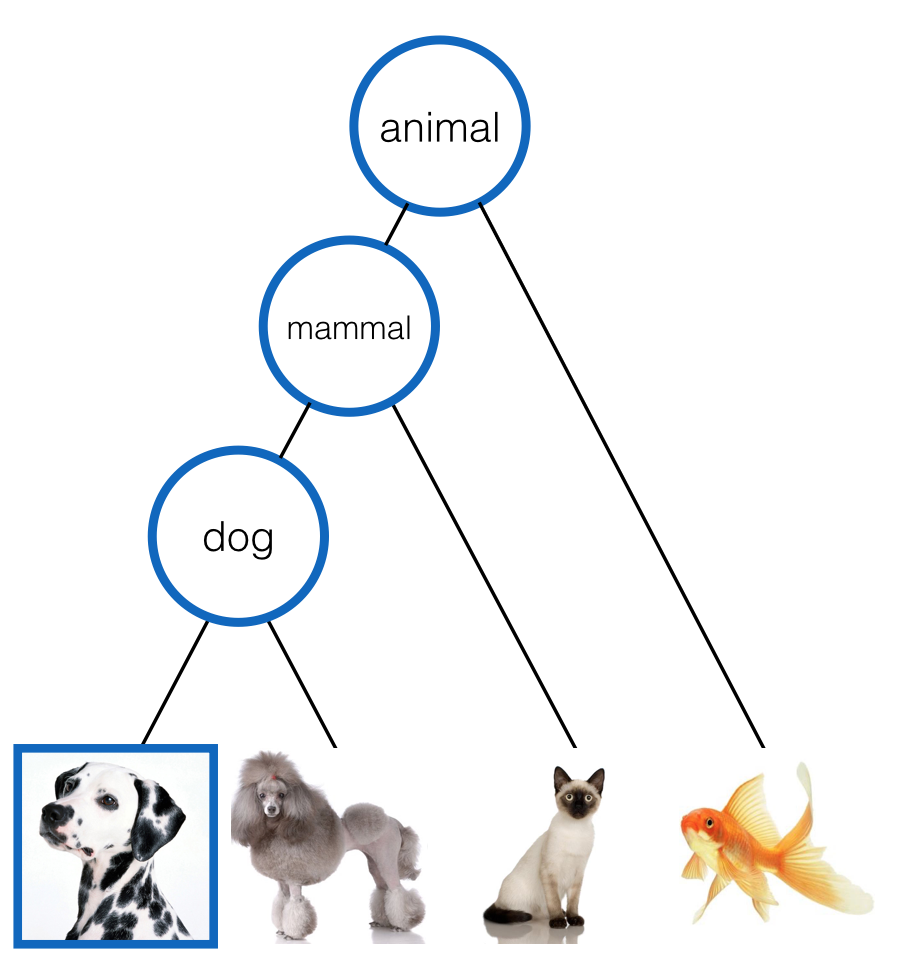
\includegraphics[scale = .4]{taskhierarchy}
\end{center}
\caption{Stimulus hierarchy used in experiment 1. The goal space and answer space contained the four object hidden behind gates (the nodes of the tree). The question space, however, was restricted to the highlighted nodes, proceeding up the hierarchy. This allows us to test the extent to which the answerer infers questioner goals. For example, both the dalmatian and poodle would be truthful responses to the explicit question `dog?' but only one is the true goal.}
\label{fig:taskhierarchy}
\end{figure}

\section{Experiment 1: \\ Questions and answers in a hierarchical world}

	\begin{figure*}[t!]
\begin{center}
\includegraphics[scale = .52]{explicit_questioner.jpeg}
\includegraphics[scale = .52]{pragmatic_answerer.jpeg}
\end{center}
\caption{These plots show our results from experiment 1, compared with the predictions of our best-performing models for both questioner and answerer behavior. We find that there is no significant difference between the explicit questioner and pragmatic questioner in this task, but that the pragmatic answerer accounts for the qualitative patterns in the response data much better than the explicit answerer.}
\label{fig:exp1res}
\end{figure*}

	While there is extensive evidence that answerers are sensitive to questioner goals and context, the novel prediction of our model is about \emph{questioner behavior}. If the pragmatic answerer uses the question itself as a signal about which underlying goal is currently at play, the questioner should choose questions that make their underlying intentions most clear.  In order to test how questioners choose questions when faced with a decision problem, and how answerers choose answers under uncertainty about this decision problem, we designed a guessing-game task played by two players: a questioner and an answerer. In this game, $4$ animals (a dalmatian, a poodle, a siamese cat, and a goldfish) were hidden behind $4$ gates. Note that these animals correspond to different levels in a class hierarchy (see Fig. \ref{fig:taskhierarchy}). The questioner was given a private goal of finding one of the objects (e.g. `find the poodle'), and the answerer had privileged information about the exact locations of each object. Before choosing a gate, the questioner could ask the answerer a single question, chosen from a restricted set of options, and the answerer could respond to this question by revealing the object behind a single gate. 
	


\subsubsection{Participants} We recruited 125 participants between the ages of 20 and 75 from Amazon Mechanical Turk to participate in this task. Each participant provided responses for four trials in the role of the questioner (corresponding to the four goals), and four trials in the role of the answerer (corresponding to the four possible questions). They were compensated 50\textcent \, for their work, and the median completion time was 4.06 minutes. Twelve participants were excluded due to self-reported confusion about the task instructions.

\subsubsection{Stimuli \& Procedure} In terms of our model specification, the world space $\mathcal{W}$ was the set of $4! = 24$ possible assignments of four objects to four gates. The goal space $\mathcal{G}$ was the set of four objects that the questioner could be trying to find (the leaves of the tree in Fig. \ref{fig:taskhierarchy}). The answer space $\mathcal{A}$ was the set of four gates that the answerer could possibly reveal. The key constraint in the task, however, was that the questioner must choose from a \emph{restricted set of questions}: they may be trying to find the goldfish, but cannot directly ask `where is the goldfish?' The question space $\mathcal{Q}$ contained the set of highlighted nodes in the hierarchy: `dalmatian?', `dog?', `mammal?', and `animal?'.



In the questioner block, players were presented with a private goal from $\mathcal{G}$, like ``find the poodle!'' and prompted to select a question from a drop-down menu containing elements of $\mathcal{Q}$ that would best help them find it. In the answerer block, players were shown which item was behind which gate and were told that the other player had asked a question from $\mathcal{Q}$. They were prompted to select a gate from a drop-down menu that would be most helpful for the questioner, keeping in mind their constraints. In order to collect responses for all elements of $\mathcal{G}$ and $\mathcal{Q}$, the order of� the questioner and answerer blocks was randomly assigned within participants, and the order of stimuli within these blocks was also randomized\footnote{All materials are available at \url{https://github.com/hawkrobe/Q\_and\_A/tree/master/experiment1/versions/experiment1\_short}}. 

\subsubsection{Results}

Results for the questioner role are shown with our model predictions in Figure \ref{fig:exp1res}(a). We find that questioners systematically prefer different questions given different goals, even as those questions become less explicitly informative. Chi-squared tests over the four response distributions each show a significant divergence from uniform. Questioners ask about the `dalmatian' given the  dalmatian goal, $\chi^2(3) = 161, p < .001$, about the `dog' given the poodle goal, $\chi^2(3) = 250, p <.001$, about the `mammal' given the cat goal, $\chi^2(3) = 25, p <.001$, and equally about the `mammal' and `animal' when given the goldfish goal, $\chi^2(3) = 44, p <.001$. This pattern broadly shows that questioners pick the lowest node in the question hierarchy that contains their goal item. 

Results for the answerer role are shown in Figure \ref{fig:exp1res}(b). Here, we find that answerers are highly sensitive to the constraints of the questioner, giving information about the dalmatian when asked about a `dalmatian', $\chi^2(3) = 258, p <.001$, about the poodle when asked about a `dog', $\chi^2(3) = 110, p <.001$, about the cat when asked about a `mammal', $\chi^2(3) = 40, p<.001$, and equally about the cat and the goldfish when asked about an `animal'. Under an explicit interpretation of the question, revealing the dalmatian and the poodle would both be perfectly acceptable answers to a question about a `dog', but answerers strongly prefer to give the location of the poodle.  

\begin{figure}[t!]
\begin{center}
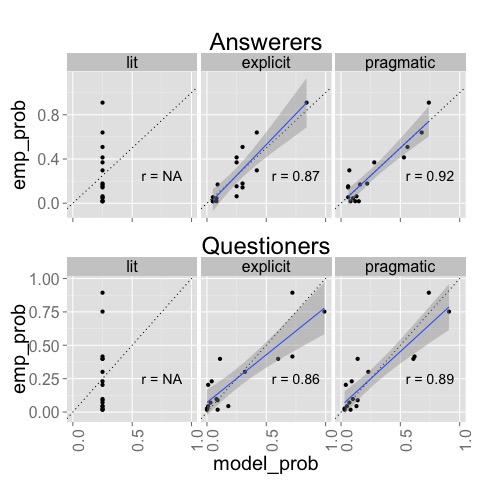
\includegraphics[scale=.5]{model_fits_grid.jpeg}
\end{center}
\caption{Full space of models, and their correlations with the data from Experiment 1. The questioner models in the second row reason about the answerers directly above them in the top row, and the pragmatic answerer reasons about the explicit questioner. Note that the explicit answerer model was fit using one rationality parameter, the explicit questioner was fit using two optimality parameters, the pragmatic answerer was fit using four parameters, and these parameters were fixed in the pragmatic questioner \todo[inline]{RDH: There needs to be more discussion of parameter fitting in the body -- the fact that the better models just have more parameters is too easy a target! Maybe if we propagate up the best vals, so that each model only has to fit one or two to its own data?}}
\label{fig:model_space}
\end{figure}

\subsubsection{Model comparison}

We now compare these results to the predictions of our family of models (Fig. \ref{fig:model_space}). At the very simplest level, our \emph{literal answerer} yields a uniform distribution over the four answers that are the case in the given world. This has important consequences for the corresponding \emph{literal questioner} model: when this questioner reasons about which question would generate the most helpful answer from the literal answerer, they find no differences, and therefore have no preference over which question to ask. The predictions of this model, plotted against our empirical results, are shown in the left-hand column of Fig. \ref{fig:model_space}. Based on the results presented above, this is clearly not how questioners and answerers behave and we will not consider the literal models further.

We now turn to our two remaining questioner models. Since the explicit questioner is nested two levels inside the pragmatic questioner, and each agent could in principle be associated with a free rationality parameter, we must consider model complexity when making comparisons. To put them on equal ground, we reduce the pragmatic questioner's rationality parameters to two: one used by all levels of questioners, and one for all levels of answerers. For each model, we tuned the two parameters to maximize the correlation between model and data. This yielded a model-data correlation of $r = 0.86$ for the explicit questioner and correlation of $r = 0.89$ for the pragmatic questioner. Although the pragmatic model has a slightly higher fit, the two models do not qualitatively differ in their predictions, so we limit our further discussion to the theoretically simpler explicit questioner. 

This model's predictions for each response distribution are shown in Fig. \ref{fig:exp1res}(a). Although the magnitude of its predictions are not in perfect alignment with the magnitude of the data, we see that it captures most of the interesting qualitative patterns of the data. In particular, it captures the modal response for each qud, and roughly tracks the ranking in each quadrant. We also note some interesting discrepancies. For instance, our model assigns highly different response probabilities for `animal' and `mammal' in the goldfish qud, when our participants preferred them equally. We will discuss some accounts for this discrepancy in the general discussion below.

Finally, we turn to our two answerer models. 
At a slightly higher level of sophistication, we have an \emph{explicit answerer}, which is equally likely to give the location of all nodes under the explicit class mentioned in the question (e.g. \emph{dog} or \emph{animal}). This model produces the answerer predictions depicted in Figure \ref{fig:model_space}(b), which successfully down-weights the least relevant alternatives, giving a model-data correlation of $r = 0.85$ \todo[inline]{stats}, with only one free (optimality) parameter, but cannot reproduce some important qualitative symmetries between the explicitly relevant alternatives. For example, it is equally likely to respond `dalmatian' and `poodle' when asked about the `dog', whereas participants significantly preferred `poodle.' The \emph{pragmatic answerer} model, which uses the question utterance to infer the questioner's underlying goal, is able to break this symmetry, for an overall fit of $r = 0.95$ \dots \todo[inline]{depends on how we reuse parameters}


\section{Related work}

Our account of question and answer behavior ultimately converges on a similar solution as contemporary decision theoretic or game theoretic accounts in linguistics. These theories were a response to early work on question and answer semantics, which focused on the notion of informativeness. In Groenendijk \& Stokhof's \citeyear{GroenendijkStokhof84_SemanticsOfQuestions} theory of question and answer semantics, asking a question induces a partition over the space of possible worlds, where each cell of the partition corresponds to a possible answer. An answer, then, consists of eliminating cells in this partition, and the most useful answers are those that eliminate all relevant alternatives to the true world. However, as van Rooy \cite{VanRooy03_QuestioningDecisionProblems} and others \cite{Ginzburg95_ResolvingQuestions} have pointed out, this predicts that \emph{wh}-questions like ``Where can I buy an Italian newspaper?'' can only be fully resolved by exhaustively mentioning whether or not such a newspaper can be bought at each possible location. Clearly, this is not the case: a single nearby location would suffice. These theories also cannot account for other contextual variation in what counts as a useful answer, such as questions like ``where are you?'' 

% More recent theories have tried to fix these problems by introducing some consideration of the questioner's goals. van Rooy \citeyear{VanRooy03_QuestioningDecisionProblems}, for instance, formalizes these goals as a decision problem faced by the questioner. A useful answer under this decision theoretic account is one that maximizes the expected value of the questioner's decision problem. A useful question is one that induces a sufficiently fine-grained partition, optimally distinguishing the worlds relevant to the decision problem. While this framework elegantly accounts for the context-dependence and relevance-maximization of question and answer behavior, it assumes that the questioner's decision problem is known \emph{a priori} by the answerer. If this were the case, the act of asking questions would seem irrelevant: why wouldn't the answerer directly tell the questioner which action to take? 

\section{General discussion}
\label{sec:gd}

Humans are experts at inferring the intentions of other agents from their actions \cite{TomaselloCarpenter___Moll05_IntentionsCulturalCognition}. Given simple motion cues, for example, we are able to reliably discern high-level goals such as chasing, fighting, courting, or playing \cite{BarrettToddMillerBlythe05_IntentionFromMotionCues, HeiderSimmel44_ApparentBehavior}. Experiments in psycholinguistics have shown that this expertise extends to speech acts as well.  Behind every question lies some goal or intention. This could be an intention to obtain an explicit piece of information (``Where can I get a newspaper?''), signal some common ground (``Did you see the game last night?''), test the answerer's knowledge (``If I add these numbers together, what do I get?''), politely request the audience to take some action (``Could you pass the salt?''), or just to make open-ended small talk (``How was your weekend?''). These wildly different intentions seem to warrant different kinds of answers, even if the explicit question is expressed using the same words.

In this paper we have presented computational-level evidence that answerer behavior is best described by a pragmatic model that reasons about questioner intentions, using the question utterance as a signal. Furthermore, we showed that questioner behavior is best described by a model that reasons about a lower-level explicit answerer. This analysis provides a novel perspective on the role of questions in dialogues: it is well-accepted under the Gricean view that answerers strive to be relevant, but we find that there is also a burden placed on the questioner to provide sufficient information about should be considered relevant in the first place. 

There are some pros and cons to the artificially restricted question space in our experiment design. On one hand, this seems to distance the behavior of participants from the types of questions and answers they would make using natural language. On the other hand, this restriction was crucial in allowing us to compare the informativeness of different questions, serving as a minimal test: when necessary, questioners can choose an optimally informative signal. However, it is worth observing that many conversational scenarios in everyday usage feature natural restrictions on the set of things one can ask about, due to politeness, salience, time cost, and other factors. We must choose our questions carefully. 

\bibliographystyle{apacite}

\setlength{\bibleftmargin}{.125in}
\setlength{\bibindent}{-\bibleftmargin}

\bibliography{bibs}


\end{document}
